\section{Preventivo}
%parte di introduzione%
Sigle identificative per i ruoli indicati nelle tabelle e nei grafici
\begin{itemize}
    \item RE: Responsabile;
    \item AM: Amministratore;
    \item AN: Analista;
    \item PT: Progettista;
    \item PR: Programmatore;
    \item VE: Verificatore.
\end{itemize}
Il costo orario associato a ciascun ruolo:

{
	\rowcolors{2}{grigetto}{white}
	\renewcommand{\arraystretch}{2}
	\centering
	\begin{longtable}{ C{2cm} C{3cm}}
		\rowcolor{rossoep}
		\textcolor{white}{\textbf{Ruolo}} & \textcolor{white}{\textbf{Costo per ora espresso in euro}}\\	
        
        Responsabile & 30\\
        Amministratore & 20\\
        Analista & 25\\
        Progettista & 22\\
        Programmatore & 15\\
        Verificatore & 15\\
		
	\end{longtable}
}

\subsection{Fase di Analisi}

\subsubsection{Divisione Oraria}
La seguente tabella §5.1.1 rappresenta la distribuzione oraria dei ruoli per ogni componente del gruppo.
{
	\rowcolors{2}{grigetto}{white}
	\renewcommand{\arraystretch}{2}
	\centering
	\begin{longtable}{ C{5cm} C{1cm} C{1cm} C{1cm} C{1cm} C{1cm} C{1cm} C{3cm}}
		\rowcolor{rossoep}
		\textcolor{white}{\textbf{Nome membro del gruppo}} & \textcolor{white}{\textbf{RE}} & \textcolor{white}{\textbf{AM}} & \textcolor{white}{\textbf{AN}} & \textcolor{white}{\textbf{PT}} & \textcolor{white}{\textbf{PR}} & \textcolor{white}{\textbf{VE}} & \textcolor{white}{\textbf{Ore complessive}}\\	
        
        
        Christian Mattei     & - & 7 & 12 & - & - & 11 & 30 \\
        Davide Lazzaro       & - & 5 & 16 & - & - & 9 & 30 \\
        Emanuele Cisotto     & - & - & 21 & - & - & 9 & 30 \\
        Enrico Salmaso       & 15 & 2 & 8  & - & - & 5 & 30 \\
        Federico Perin       & - & - & 21 & - & - & 9 & 30 \\
        Francesco Drago      & - & 7 & 16 & - & - & 7 & 30 \\
        Riccardo Baratin     & - & 5 & 11 & - & - & 14 & 30 \\
        Tommaso Azzalin      & 4 & 12 & 9  & - & - & 5 & 30 \\
        \textbf{Ore totali ruolo} & 19 & 38 & 114 & - & - & 69 & 240 \\
		
	\end{longtable}
}

La quantità di ore che ciascun componente del gruppo ha svolto per ogni ruolo viene rappresentata nel seguente istogramma:

\begin{figure}[h]
%	\centering
%	\includegraphics[scale=0.45]{sezioni/Istogrammi/}
%	\caption{Istogramma della disposizione ore per ruolo di ciascun componente del periodo di analisi}
\end{figure}

\subsubsection{Costo Risultate}
La seguente tabella §5.1.2 rappresenta, per ruolo, le ore totali investite e il corrispondente costo in euro.
{
	\rowcolors{2}{grigetto}{white}
	\renewcommand{\arraystretch}{2}
	\centering
	\begin{longtable}{ C{3cm} C{2cm} C{4cm}}
		\rowcolor{rossoep}
		\textcolor{white}{\textbf{Ruolo}} & \textcolor{white}{\textbf{Totale ore}} & \textcolor{white}{\textbf{Costo Ruolo in euro}}\\	
        
        Responsabile & 19 & 570\\
        Amministratore & 38 & 760\\
        Analista & 114 & 2.850 \\
        Progettista & 0 & 0 \\
        Programmatore & 0 & 0 \\
        Verificatore & 69 & 1.035 \\
        \textbf{Totale} & 240 & 5.215 \\
		
	\end{longtable}
}

La quantità di ore totali di ciascun ruolo viene rappresentata nel seguente aerogramma:

\begin{figure}[h]
%	\centering
%	\includegraphics[scale=0.45]{sezioni/Aerogrammi/}
%	\caption{Suddivisione ore per ruolo del periodo di analisi}
\end{figure}

\subsection{Progettazione architetturale}

\subsubsection{Divisione Oraria}
La seguente tabella §5.2.1 rappresenta la distribuzione oraria dei ruoli per ogni componente del gruppo.
{
	\rowcolors{2}{grigetto}{white}
	\renewcommand{\arraystretch}{2}
	\centering
	\begin{longtable}{ C{5cm} C{1cm} C{1cm} C{1cm} C{1cm} C{1cm} C{1cm} C{3cm}}
		\rowcolor{rossoep}
		\textcolor{white}{\textbf{Nome membro del gruppo}} & \textcolor{white}{\textbf{RE}} & \textcolor{white}{\textbf{AM}} & \textcolor{white}{\textbf{AN}} & \textcolor{white}{\textbf{PT}} & \textcolor{white}{\textbf{PR}} & \textcolor{white}{\textbf{VE}} & \textcolor{white}{\textbf{Ore complessive}}\\	
        
        Christian Mattei & 5 & & & 14 & 10 & 4 & 33\\
        Davide Lazzaro & 8 & & & 18 & & 7 & 33 \\
        Emanuele Cisotto & & 8 & & 10 & 5 & 6 & 32 \\
        Enrico Salmaso & & 10 & 6 & 10 & & 6 & 29 \\
        Federico Perin & & 6 & & 5 & 7 & 13 &  31\\
        Francesco Drago & & & 13 & 5 & 7 & 6 & 31 \\
        Riccardo Baratin & 6 & & & & 17 & 8 & 31\\
        Tommaso Azzalin & & & 8 & 7 & & 16 & 31\\
        \textbf{Ore totali ruolo} & 19 & 24 & 27 & 69 & 46 & 66 & \\
		
	\end{longtable}
}

La suddivisione di quante ore ha svolto ciascun componente del gruppo per ogni ruolo viene rappresentata nel seguente istogramma:

\begin{figure}[h]
	\centering
	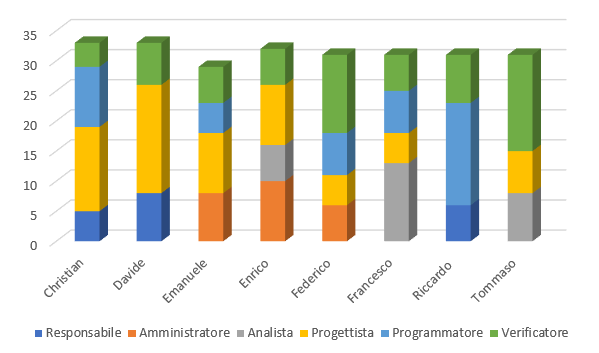
\includegraphics[scale=3]{sezioni/Istogrammi/IstogrammaProgettArchitetturale.png}
	\caption{Istogramma della disposizione ore per ruolo di ciascun componente del periodo di progettazione architetturale}
\end{figure}

\subsubsection{Costo Risultate}
La seguente tabella §5.2.2 rappresenta, per ruolo, le ore totali investite e il corrispondente costo in euro.
{
	\rowcolors{2}{grigetto}{white}
	\renewcommand{\arraystretch}{2}
	\centering
	\begin{longtable}{ C{3cm} C{2cm} C{4cm}}
		\rowcolor{rossoep}
		\textcolor{white}{\textbf{Ruolo}} & \textcolor{white}{\textbf{Totale ore}} & \textcolor{white}{\textbf{Costo Ruolo in euro}}\\	
        
        Responsabile & 19 & 570 \\
        Amministratore & 24 & 480 \\
        Analista & 27 & 675 \\
        Progettista & 69 & 1518 \\
        Programmatore & 46 & 690 \\
        Verificatore & 66 & 990 \\
        \textbf{Totale} & 251 & 4.923 \\
		
	\end{longtable}
}

La suddivisione della quantità di ore totali di ciascun ruolo viene rappresentata nel seguente aerogramma:

\begin{figure}[h]
	\centering
	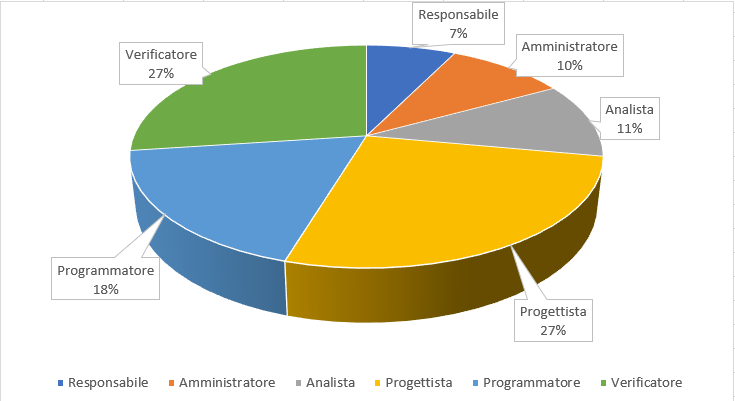
\includegraphics[scale=2]{sezioni/Aerogrammi/AerogrammaProgettArchitetturale.png}
	\caption{Suddivisione ore per ruolo del periodo di progettazione architetturale}
\end{figure}

\subsection{Progettazione di dettaglio e codifica}

\subsubsection{Divisione Oraria}
La seguente tabella §5.3.1 rappresenta la distribuzione oraria dei ruoli per ogni componente del gruppo.
{
	\rowcolors{2}{grigetto}{white}
	\renewcommand{\arraystretch}{2}
	\centering
	\begin{longtable}{ C{5cm} C{1cm} C{1cm} C{1cm} C{1cm} C{1cm} C{1cm} C{3cm}}
		\rowcolor{rossoep}
		\textcolor{white}{\textbf{Nome membro del gruppo}} & \textcolor{white}{\textbf{RE}} & \textcolor{white}{\textbf{AM}} & \textcolor{white}{\textbf{AN}} & \textcolor{white}{\textbf{PT}} & \textcolor{white}{\textbf{PR}} & \textcolor{white}{\textbf{VE}} & \textcolor{white}{\textbf{Ore complessive}}\\	
        
        Christian Mattei & & 10 & & 12 & 15 & 10 & 47\\
        Davide Lazzaro & 6 & & & 10 & 15 & 16 & 47\\
        Emanuele Cisotto & & 5 & & 13 & 16 & 13 & 47 \\
        Enrico Salmaso & & 4 & & 11 & 18 & 14 & 47\\
        Federico Perin & & 8 & & 8 & 19 & 12 & 47\\
        Francesco Drago & 10 & & & 7 & 17 & 13 & 47\\
        Riccardo Baratin & & 3 & & 12 & 19 & 13 & 47\\
        Tommaso Azzalin & 10 & & & 10 & 17 & 10 & 47 \\
        \textbf{Ore totali ruolo} & 26 & 30 & & 83 & 136 & 101 & 376\\
		
	\end{longtable}
}

La suddivisione di quante ore ha svolto ciascun componente del gruppo per ogni ruolo viene rappresentata nel seguente istogramma:

\begin{figure}[h]
	\centering
	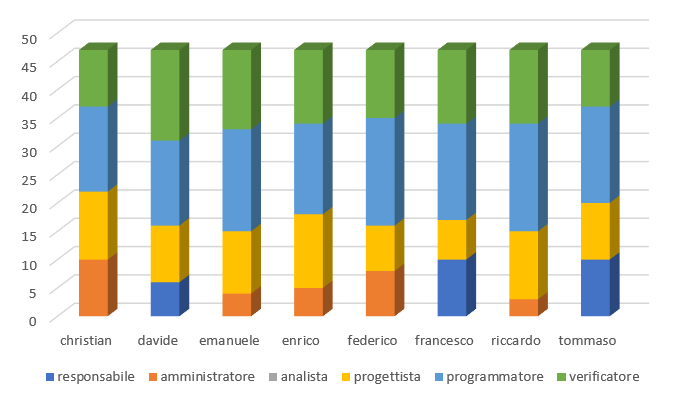
\includegraphics[scale=2]{sezioni/Istogrammi/IstogrammaDiDettaglio.png}
	\caption{Istogramma della disposizione ore per ruolo di ciascun componente del periodo di progettazione di dettaglio e codifica}
\end{figure}

\subsubsection{Costo Risultate}
La seguente tabella §5.3.2 rappresenta, per ruolo, le ore totali investite e il corrispondente costo in euro.
{
	\rowcolors{2}{grigetto}{white}
	\renewcommand{\arraystretch}{2}
	\centering
	\begin{longtable}{ C{3cm} C{2cm} C{4cm}}
		\rowcolor{rossoep}
		\textcolor{white}{\textbf{Ruolo}} & \textcolor{white}{\textbf{Totale ore}} & \textcolor{white}{\textbf{Costo Ruolo in euro}}\\	
        
        Responsabile & 26 & 780 \\
        Amministratore & 30 & 600 \\
        Analista & 0 & 0 \\
        Progettista & 83 & 1.826 \\
        Programmatore & 136 & 2.040 \\
        Verificatore & 101 & 1.515\\
        \textbf{Totale} & 376 & 6.761 \\
		
	\end{longtable}
}

La suddivisione della quantità di ore totali di ciascun ruolo viene rappresentata nel seguente aerogramma:

\begin{figure}[h]
	\centering
	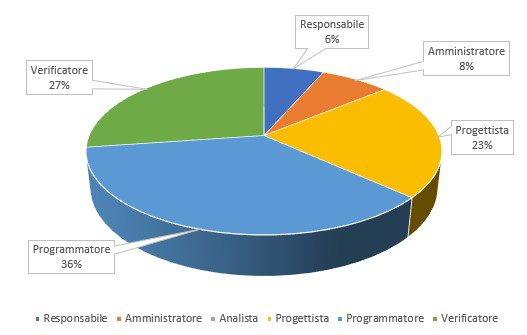
\includegraphics[scale=2]{sezioni/Aerogrammi/AerogrammaDiDettaglio.png}
	\caption{Suddivisione ore per ruolo del periodo di Progettazione di dettaglio e codifica}
\end{figure}

\subsection{Validazione e collaudo}

\subsubsection{Divisione Oraria}
La seguente tabella §5.4.1 rappresenta la distribuzione oraria dei ruoli per ogni componente del gruppo.
{
	\rowcolors{2}{grigetto}{white}
	\renewcommand{\arraystretch}{2}
	\centering
	\begin{longtable}{ C{5cm} C{1cm} C{1cm} C{1cm} C{1cm} C{1cm} C{1cm} C{3cm}}
		\rowcolor{rossoep}
		\textcolor{white}{\textbf{Nome membro del gruppo}} & \textcolor{white}{\textbf{RE}} & \textcolor{white}{\textbf{AM}} & \textcolor{white}{\textbf{AN}} & \textcolor{white}{\textbf{PT}} & \textcolor{white}{\textbf{PR}} & \textcolor{white}{\textbf{VE}} & \textcolor{white}{\textbf{Ore complessive}}\\	
        
        Christian Mattei & & & 7 & & 4 & 8 & 19\\
        Davide Lazzaro & & 4 & & 5 & & 10 & 19\\
        Emanuele Cisotto & & & & 6 & 5 & 9 & 20 \\
        Enrico Salmaso & 5 & & & & 6 & 12 & 23\\
        Federico Perin & 6 & & & & 7 & 8 & 21\\
        Francesco Drago & & 6 & & & 9 & 6 & 21\\
        Riccardo Baratin & & 5 & & & 6 & 10 & 21\\
        Tommaso Azzalin & & & 4 & 10 & & 7 & 21\\
        \textbf{Ore totali ruolo} & 11 & 15 & 11 & 21 & 37 & 69 & \\
		
	\end{longtable}
}


La suddivisione di quante ore ha svolto ciascun componente del gruppo per ogni ruolo viene rappresentata nel seguente istogramma:

\begin{figure}[h]
	\centering
	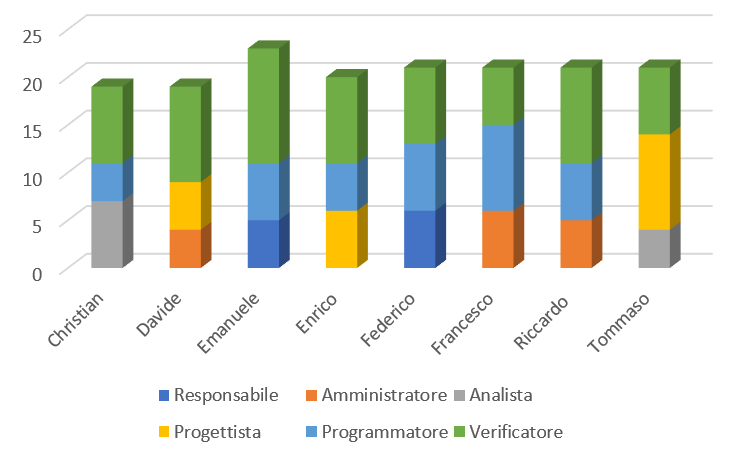
\includegraphics[scale=2.5]{sezioni/Istogrammi/IstogrammaValidazione.png}
	\caption{Istogramma della disposizione ore per ruolo di ciascun componente del periodo di validazione e collaudo}
\end{figure}

\subsubsection{Costo Risultate}
La seguente tabella §5.4.2 rappresenta, per ruolo, le ore totali investite e il corrispondente costo in euro.
{
	\rowcolors{2}{grigetto}{white}
	\renewcommand{\arraystretch}{2}
	\centering
	\begin{longtable}{ C{3cm} C{2cm} C{4cm}}
		\rowcolor{rossoep}
		\textcolor{white}{\textbf{Ruolo}} & \textcolor{white}{\textbf{Totale ore}} & \textcolor{white}{\textbf{Costo Ruolo in euro}}\\	
        
        Responsabile & 11 & 330\\
        Amministratore & 15 & 300 \\
        Analista & 11 & 275\\
        Progettista & 21 & 462\\
        Programmatore & 37 & 555\\
        Verificatore & 69 & 1035\\
        \textbf{Totale} & 169 & 2457\\
		
	\end{longtable}
}

La suddivisione della quantità di ore totali di ciascun ruolo viene rappresentata nel seguente aerogramma:

\begin{figure}[h]
	\centering
	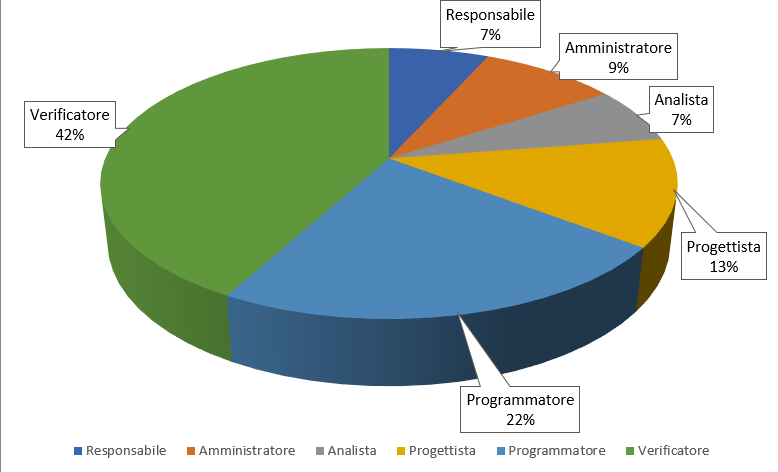
\includegraphics[scale=2.5]{sezioni/Aerogrammi/AerogrammaValidazione.png}
	\caption{Suddivisione ore per ruolo del periodo di validazione e collaudo}
\end{figure}


\clearpage
\subsection{Preventivo finale}
\subsubsection{Divisione oraria complessiva}
{
	\rowcolors{2}{grigetto}{white}
	\renewcommand{\arraystretch}{2}
	\centering
	\begin{longtable}{ C{5cm} C{1cm} C{1cm} C{1cm} C{1cm} C{1cm} C{1cm} C{3cm}}
		\rowcolor{rossoep}
		\textcolor{white}{\textbf{Nome membro del gruppo}} & \textcolor{white}{\textbf{RE}} & \textcolor{white}{\textbf{AM}} & \textcolor{white}{\textbf{AN}} & \textcolor{white}{\textbf{PT}} & \textcolor{white}{\textbf{PR}} & \textcolor{white}{\textbf{VE}} & \textcolor{white}{\textbf{Ore complessive}}\\	
        
        Christian Mattei & & & & & & & \\
        Davide Lazzaro & & & & & & & \\
        Emanuele Cisotto & & & & & & & \\
        Enrico Salmaso & & & & & & & \\
        Federico Perin & & & & & & & \\
        Francesco Drago & & & & & & & \\
        Riccardo Baratin & & & & & & & \\
        Tommaso Azzalin & & & & & & & \\
        \textbf{Ore totali ruolo} & & & & & & & \\
		
	\end{longtable}
}
\subsubsection{Costo complessivo per ruolo}
{
	\rowcolors{2}{grigetto}{white}
	\renewcommand{\arraystretch}{2}
	\centering
	\begin{longtable}{ C{3cm} C{2cm} C{4cm}}
		\rowcolor{rossoep}
		\textcolor{white}{\textbf{Ruolo}} & \textcolor{white}{\textbf{Totale ore}} & \textcolor{white}{\textbf{Costo Ruolo in euro}}\\	
        
        Responsabile & & \\
        Amministratore & & \\
        Analista & & \\
         Progettista & & \\
        Programmatore & & \\
        Verificatore & & \\
		
	\end{longtable}
}

\subsubsection{Costo complessivo}
{
	\rowcolors{2}{grigetto}{white}
	\renewcommand{\arraystretch}{2}
	\centering
	\begin{longtable}{ C{5cm} C{5cm}}
		\rowcolor{rossoep}
		\textcolor{white}{\textbf{Fase}} & \textcolor{white}{\textbf{Costo Fase}}\\	
		
		Progettazione Architetturale &  \\
		Progettazione di Dettaglio e Codifica & \\
		Validazione e Collaudo & \\
		\textbf{Totale} & \\
		
	\end{longtable}
}



